% Created 2024-08-03 Sat 16:24
% Intended LaTeX compiler: pdflatex
\documentclass[10pt]{article}
% =================================BASE====================================%
\usepackage[left=2cm,right=2cm,top=2cm,bottom=2cm]{geometry} % Marges
\usepackage[T1]{fontenc} % Nécessaire avec FrenchBabel
\usepackage[utf8]{inputenc} % Important pour symboles Francophones, é,à,etc
\usepackage{csquotes} % Recommandé par PDFLatex lors de la compilation. 

% Calligraphie
%\usepackage{pxfonts} % Met le texte ET les maths en Palatino + donne accès à des symboles math
%\usepackage{palatino} % Cette commande met seulement le texte en police palatino
\usepackage{lmodern} % Pour les maths? Lmodern pour les maths
\usepackage{cfr-lm}
% Use lmodern for sans-serif
\usepackage{mathrsfs} % Permet la command \mathscr (Lettres attachées genre) \mathscr(B)

% Bibliographie
%\usepackage[backend=bibtex,style=phys,sorting=ynt]{biblatex}
\usepackage[backend=biber,sorting=ynt,style=authoryear]{biblatex} % N'est pas utilisé par le compilateur org-mode, mais NÉCESSAIRE. Voir le fichier init.el pour changer le style. 
\addbibresource{master-bibliography.bib}


\usepackage{amsmath, amssymb, amsthm} % Symb. math. (Mathmode+Textmode) + Beaux théorèmes.
\usepackage{mathtools,cancel,xfrac} % Utilisation de boîtes \boxed{} + \cancelto{}{}, xfrac
\usepackage{graphicx, wrapfig} % Géstion des figures.
\usepackage{hyperref} % Permettre l'utilisation d'hyperliens.
\usepackage{color} % Permettre l'utilisation des couleurs.
\usepackage{colortbl} % Color tables
\usepackage[dvipsnames]{xcolor} % Couleurs avancées.

% Physique
\usepackage{physics} % Meilleur package pour physicien. 

% Style
\usepackage{lipsum} % For fun
\usepackage{tikz} % Realisation de figures TIKZ.
\usetikzlibrary{arrows.meta,bending} % Arrow heads 
\usepackage{empheq} % Boite autour de MULTIPLE équations
\usepackage{bbding}

% Français
\usepackage[french]{babel} % Environnements en Français.

\usepackage{titling} % Donne accès à \theauthor, \thetitle, \thedate

% ==============================BASE-(END)=================================%





% ================================SETTINGS=================================%
% Pas d'indentation en début de paragraphe :
\setlength\parindent{0pt}
\setlength{\parskip}{0.15cm}

% Tableaux/tabular
% Espace vertical dans les tabular/tableaux
\renewcommand{\arraystretch}{1.2}
% Couleur des tableaux/tabular
% \rowcolors{3}{violet!5}{}

% Couleurs de hyperliens :
\definecolor{mypink}{RGB}{147, 0, 255}
\hypersetup{colorlinks, 
             filecolor=mypink,
             urlcolor=mypink, 
             citecolor=mypink, 
             linkcolor=mypink, 
             anchorcolor=mypink}


% Numéros d'équations suivent les sections :
\numberwithin{equation}{section} 

% Les « captions » sont en italique et largeur limitée
\usepackage[textfont = it]{caption} 
\captionsetup[wrapfigure]{margin=0.5cm}

% Retirer l'écriture en gras dans la table des matières
\usepackage{tocloft}
\renewcommand{\cftsecfont}{\normalfont}
\renewcommand{\cftsecpagefont}{\normalfont}

% Change bullet style
\usepackage{pifont}
\usepackage{enumitem}
%\setlist[itemize,1]{label=\ding{224}}
\setlist[itemize,1]{label=\ding{239}}
\renewcommand{\boxtimes}{\blacksquare}
% ================================SETTINGS=================================%



% ==============================NEWCOMMANDS================================%
% CQFD symbol
\renewcommand{\qedsymbol}{$\hfill\blacksquare$}

% Vecteurs de base :
\newcommand{\nvf}{\vb{\hat{n}}}
\newcommand{\evf}{\vb{\hat{e}}}
\newcommand{\ivf}{\vb{\hat{i}}}
\newcommand{\jvf}{\vb{\hat{j}}}
\newcommand{\kvf}{\vb{\hat{k}}}
\newcommand{\uu}{\vb{u}}
\newcommand{\vv}{\vb{v}}
\newcommand{\ust}{\vb{u}_{\ast}}

% Physics empty spaces 
\newcommand{\short}{\vphantom{pA}}
\newcommand{\tall}{\vphantom{pA^{x^x}_p}}
\newcommand{\grande}{\vphantom{\frac{1}{xx}}}
\newcommand{\venti}{\vphantom{\sum_x^x}}
\newcommand{\pt}{\hspace{1pt}} % One horizontal pt space

% Moyenne numérique entre deux points de grilles. 
\newcommand{\xmean}[1]{\overline{#1}^x}
\newcommand{\ymean}[1]{\overline{#1}^y}
\newcommand{\zmean}[1]{\overline{#1}^z}
\newcommand{\xymean}[1]{\overline{#1}^{xy}}

% Tilde over psi
\newcommand{\tpsi}{\tilde{\psi}}
\newcommand{\tphi}{\tilde{\phi}}

% Nota Bene env : (\ding{89})
%\newcommand{\nb}{$\boxed{\text{\footnotesize\EightStarConvex}\pt \mathfrak{N. B.}}$\hspace{4pt}}
\newcommand{\nb}{\underline{{\footnotesize\EightStarConvex}\pt $\mathfrak{N.B.}$\vphantom{p}}\hspace{3pt}}

\newcommand{\exemple}{
\parbox[center]{2.2cm}{\begin{tcolorbox}[sharp corners, rounded corners=northeast, rounded corners=southeast,
colback=Violet!2, colframe=black,
size=small, width=2cm, left=-0.25pt, bottom=-0.5pt,
arc is angular, arc=2.5mm, boxrule=0.35pt, leftrule=4pt, %bottomrule=1pt,
after={\enskip}] Exemple \end{tcolorbox}}}

\newcommand{\rad}{\text{Rad}}


\newcommand{\cqfd}{\hfill$\blacktriangleleft$}

% Define the nota bene environment
\usepackage{tcolorbox}
\newtcolorbox{notabene}{
     colback=blue!5,
     colframe=black,
     boxrule=0.5pt,
     arc=2pt,
     left=5pt,
     right=5pt,
     top=5pt,
     bottom=5pt,
}


\newcommand{\cmark}{\ding{52}}
\newcommand{\xmark}{\ding{55}}
% ==============================NEWCOMMANDS================================%



% ==============================PAGE-TITRE=================================%
% Titlepage 
\newcommand{\mytitlepage}{
\begin{titlepage}
\begin{center}
{\Huge \thesubtitle \par}
\vspace{2cm}
{\Huge \MakeUppercase{\thetitle} \par}
\vspace{2cm}
RÉALISÉ DANS LE CADRE\\ D'UN PROJET POUR \par
\vspace{2cm}
{\Huge ISMER--UQAR \par}
\vspace{2cm}
{\thedate}
\end{center}
\vfill
Rédaction \\
{\theauthor}\\
\url{charles-edouard.lizotte@uqar.ca}\\
ISMER-UQAR\\
Police d'écriture : \textbf{CMU Serif Roman}
\end{titlepage}
}
% ==============================PAGE-TITRE=================================%



% =================================ENTÊTE==================================%
\usepackage{fancyhdr}
\pagestyle{fancy}
\setlength{\headheight}{13pt}
\renewcommand{\headrulewidth}{0.025pt} % Ligne horizontale en haut

\fancyhead[R]{\textit{\thetitle}}
\fancyhead[L]{\ \thepage}
\fancyfoot[R]{\textit{\theauthor}}
\fancyfoot[L]{}
\fancyfoot[C]{} 
% =================================ENTÊTE==================================%
\author{Charles-Édouard Lizotte}
\date{12/05/2023}
\title{Carnet de bord, Université McGill}
\newcommand{\thesubtitle}{Contrat Été 2023}
\hypersetup{
 pdfauthor={Charles-Édouard Lizotte},
 pdftitle={Carnet de bord, Université McGill},
 pdfkeywords={},
 pdfsubject={},
 pdfcreator={Emacs 29.4 (Org mode 9.7.8)}, 
 pdflang={French}}
\begin{document}

\mytitlepage
\tableofcontents\newpage
\section{Nouvelle formulation pour le gradient de pression}
\label{sec:org6f20907}

David nous a éclairé de sa lumière mardi à 21h43 et nous est arrivé avec un solution super simple mais efficace.
En premier lieu, on se souvient qu'on définit notre pas de temps \emph{leapfrog} de manière à ce que
\begin{equation}
 \uu^{t+1} = \underbrace{ \uu^{t-1} + (2\Delta t)\cdot \vb*{G}^t}_{\tilde{\uu}} + \gradient{\phi}.
\end{equation}

On peut décomposer notre courant en deux composantes, soit barotrope et baroclines, de sorte à retrouver
\begin{subequations}
\begin{align}
 & \tilde{\uu}_{BT} = \frac{1}{H} \sum_k^n d_k \tilde{\uu}_k, \\
 & \tilde{\uu}_{BC} = \tilde{\uu} - \tilde{\uu}_{BT}.
\end{align}
\end{subequations}

Puis à l'aide de ce courant barotrope, on peut construire une vorticité barotrope
\begin{equation}
 \tilde{\zeta}_{BT} = \kvf \cdot \qty[\curl{\tilde{\uu}_{BT}}].
\end{equation}

Mais on peut aussi calculer la vorticité de notre futur courant, de sorte à retrouver
\begin{align}
& \zeta^{t+1}_{BT} = \kvf \cdot \qty[\curl{\uu^{t+1}_{BT}}],\venti\nonumber\\
& \zeta^{t+1}_{BT} = \kvf \cdot \qty[\curl(\tilde{\uu}_{BT} + \gradient{\phi})],\venti\nonumber\\
& \zeta^{t+1}_{BT} = \kvf \cdot \qty[\curl{\tilde{\uu}_{BT}}] + \cancelto{0}{\kvf\cdot\qty[\curl{\gradient{\phi}}]}.
\end{align}
Comme le rotationnel d'un gradient est toujours nul, on arrive à la conclusion inévitable que
\begin{equation}
 \zeta^{t+1}_{BT} = \tilde{\zeta}_{BT}.
\end{equation}
La correspondance entre la vorticité relative est donnée par \(\zeta = \laplacian{\psi}\), donc on obtient une nouvelle équation de Poisson donnée par
\begin{equation}
\boxed{\hspace{0.3cm}
 \laplacian{\psi_{BT}} = \kvf \cdot \qty[\curl{\tilde{\uu}_{BT}}]
 \hspace{0.31cm}\text{avec C.F. Dirichlet}\hspace{0.31cm}
 \eval{\psi_{BT}\pt}_{x_0,\pt x_f} = \ \eval{\psi_{BT}\pt}_{y_0,\pt y_f} = 0.
\hspace{0.3cm} }
\end{equation}
Donc en trouvant \(\psi_{BT}\), on trouve aussi \(\uu_{BT}\) à l'aide de la relation avec la fonction de courant,
\begin{align}
&&u = -\pdv{\psi}{y} &&\text{et} && v = \pdv{\psi}{x}.&&
\end{align}
Puis finalement, on retrouve
\begin{align}
 \uu^{t+1} = \uu_{BT} + \uu_{BC} = \curl{\qty(\kvf\psi_{BT})} + \uu_{BC},
\end{align}
où \(\uu_{BC} = \tilde{\uu}_{BC}\) car \(\gradient{\phi}\) est une composante barotrope.
\subsection{Avantages}
\label{sec:org641c07c}
En premier lieu, cette méthode a l'avantage de ramener le problème directement aux frontières.
Mentionnons qu'en raison de la condition \emph{free slip} et \emph{no normal flow}, les frontières doivent être sur les courants opur une grille Arakawa-C (notre cas). 
En second, nous n'avons plus besoin de calculer le gradient de pression à l'aide des cette méthode.
On remplace plutôt notre variable inconnue par une fonction de courant barotrope \(\psi_{BT}\).
\subsection{Désavantages}
\label{sec:orge28c92e}
Mentionnons que cette méthode est un peu plus lente.
À trois couches, on note au moins un temps de calcul deux fois plus lent.
Comme notre objectif final est de coupler cette version du modèle avec Wavewatch III, le temps de calcul ne devrait pas être un obstable pour ce modèle-ci. 
\section{Algorithme de solution à \(\psi_{BT}\)}
\label{sec:org5604593}

La documentation de MUDPACK signalait qu'il est possible d'utiliser deux techniques pour améliorer le temps de calcul et limiter l'erreur numérique.
\subsection{Calculer la correction à la solution plutôt que la solution}
\label{sec:orgd8a9d4d}
Nous avons en main une équation différentielle elliptique quelconque.
Cette dernière peut être décrite par un opérateur \(\mathcal{L}\) linéaire qui satisfait,
\begin{align}
&&\mathcal{L}\ \qty[\phi(t)] = f(t) && \text{et} && \mathcal{L}\ \qty[\phi(t+\delta t)] = f(t+\delta t), &&
\end{align}
où la fonction \(f\) dépend de \(x,y\) de sorte que \(f(t)\) est la notation simplifiée de \(f(x,y,t)\) -- il en est de même avec \(\phi(t)\).
Il est donc possible de définir une correction \(e\pt(t,\delta t)\) tel que
\begin{align}
\mathcal{L}\ \qty[\pt e\pt(t,\delta t)\pt ] = \mathcal{L}\ \qty[ \phi(t+\delta t) - \phi(t) ] = f(t+\delta t) - f(t).
\end{align}
On peut donc solutionner \(e\pt(t,\delta t)\) au lieu de \(\phi(t)\) et faire le chemin inverse à l'aide de
\begin{equation}
\phi(t+\delta t) = \phi(t) + e\pt(t,\delta t).
\end{equation}

\textbf{N.B.} Malheureusement, j'ai essayé et le résultat était peu concluant.
Notre champ initialement calculé (\(f(t+\delta t)\)) n'est pas vraiment au temps \(t+\delta t\) en fait.
Donc il est peu aviser d'utiliser \(f(t+\delta t) - f(t)\) comme RHS de notre équation elliptique pour trouver la correction \(e\pt(t,\delta t)\).
J'en parlerai à David, car ça pourrait légitimement réduire l'erreur numérique, même si ça ne semble pas être un problème pour l'instant.
Entre temps, nous sommes revenus à la solution initiale.
Les résultats comparatifs se retrouveront dans le prochain rapport. 
\subsection{Calculer la correction à la solution plutôt que la solution (Revisité)}
\label{sec:orga5223ac}

Comme ça induisait de drôles d'erreurs (voir figure \ref{fig:orge60970c}), j'ai décidé de revisiter le problème analytiquement.

\begin{figure}[htbp]
\centering
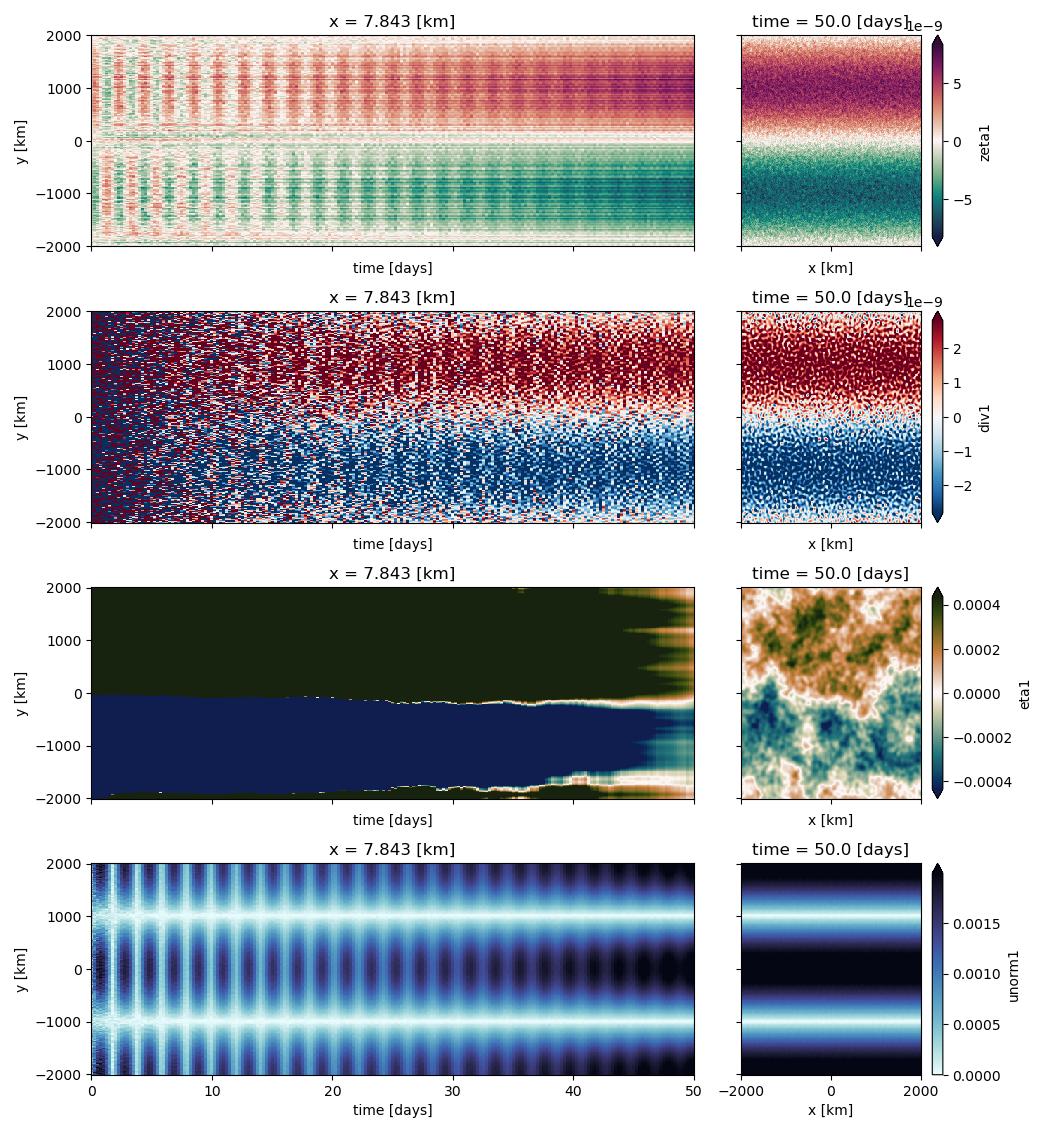
\includegraphics[width=.9\linewidth]{figures/tests/2023-05-23_hovmoller1.png}
\caption{\label{fig:orge60970c}Application de la correction à la solution plutôt que la solution elle-même dans le solveur elliptique de MUDPACK. Les résultats ne sont pas très positifs.}
\end{figure}
\subsection{Utiliser le dernier champ comme tentative initiale}
\label{sec:org4fb09d7}
Il est conseillé d'utiliser \(\phi(t)\) comme tentative initiale pour solutionner \(\phi(t+\delta t)\) au lieu d'un champ vide comme une matrice nulle, par exemple.
C'est ce que nous avons fait comme cette méthode prenait une seule ligne de code. 
\section{Considérations d'échelle sur la correction à \(\psi_{BT}\)}
\label{sec:org1eb6ceb}

Quelle est l'ordre de la correction appliquée à la fonction de courant barotrope \(\psi_{BT}\)?
Au début, les maxima gravitent autours de 4 [\(s^{-1}\)].
De leur côté, les courants océaniques atteignent ordinairement des vitesses de l'ordre de \(\order*{10^{-1}}\) à leur maxima.
Il n'est alors pas déraisonnable d'affirmer que 
\begin{equation}
\norm{\uu} = - \frac{\delta \psi}{\delta y} \Longrightarrow \frac{[\ ?\ s^{-1}\ ]}{[\simeq 3600m]} = \order{10^{-1}}.
\end{equation}
À l'aide de la puissante règle du produit croisé, on en déduit que les variations de \(\psi\) sont de l'ordre de 360 \(s^{-1}\), donc \(\order*{10^2}\).\bigskip

Si l'on met cette valeur en perspective, les corrections maximum de \(\psi\) à l'aide de MUDPACK \((\sim 3 s^{-1})\), sont de l'ordre \(\order*{1}\).
Donc nous sommes dans le royaume du pourcent, ce qui est rassurant car c'est ce que nous avions avec la correction du gradient de pression par \emph{fft}. 
\section{Bibliographie}
\label{sec:orgeabe721}
\end{document}
